\chapter{Additional data from patient with interdigitating dendritic cell sarcoma}
\label{app.303}

\begin{figure}[htp]
    \begin{center}
        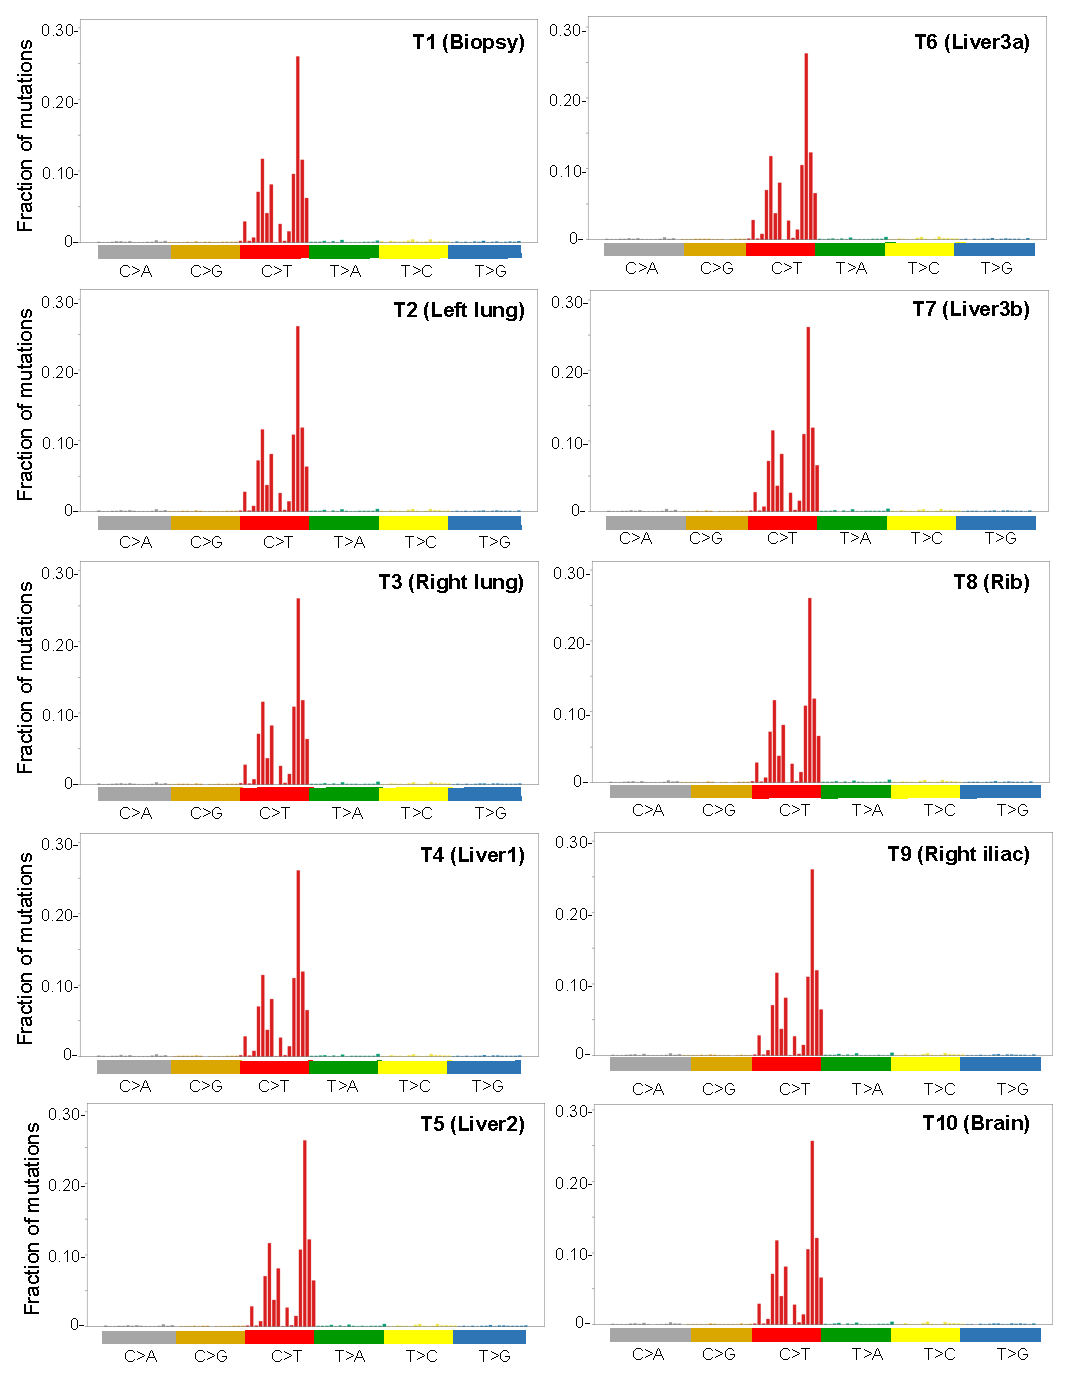
\includegraphics[width=0.84\textwidth,keepaspectratio]{images/303/mutational_spectra_by_sample}
    \end{center}
    \caption[Mutational spectra per IDCS tumor sample.]{Mutational spectra per tumor sample. Each lego plot portrays the distribution of mutations in each sample, given their trinucleotide context. The X-axis of lego plots contains 96 possible mutation types that result when the six classes of base substitutions (e.g. C\textgreater{}T) are placed in the trinucleotide context of flanking 5' and 3' bases. The Y-axis represents the fraction of base substitutions in each sample within each trinucleotide context}
    \label{fig:303:mutational_spectra_by_sample}
\end{figure}

\begin{figure}[htp]
    \begin{center}
        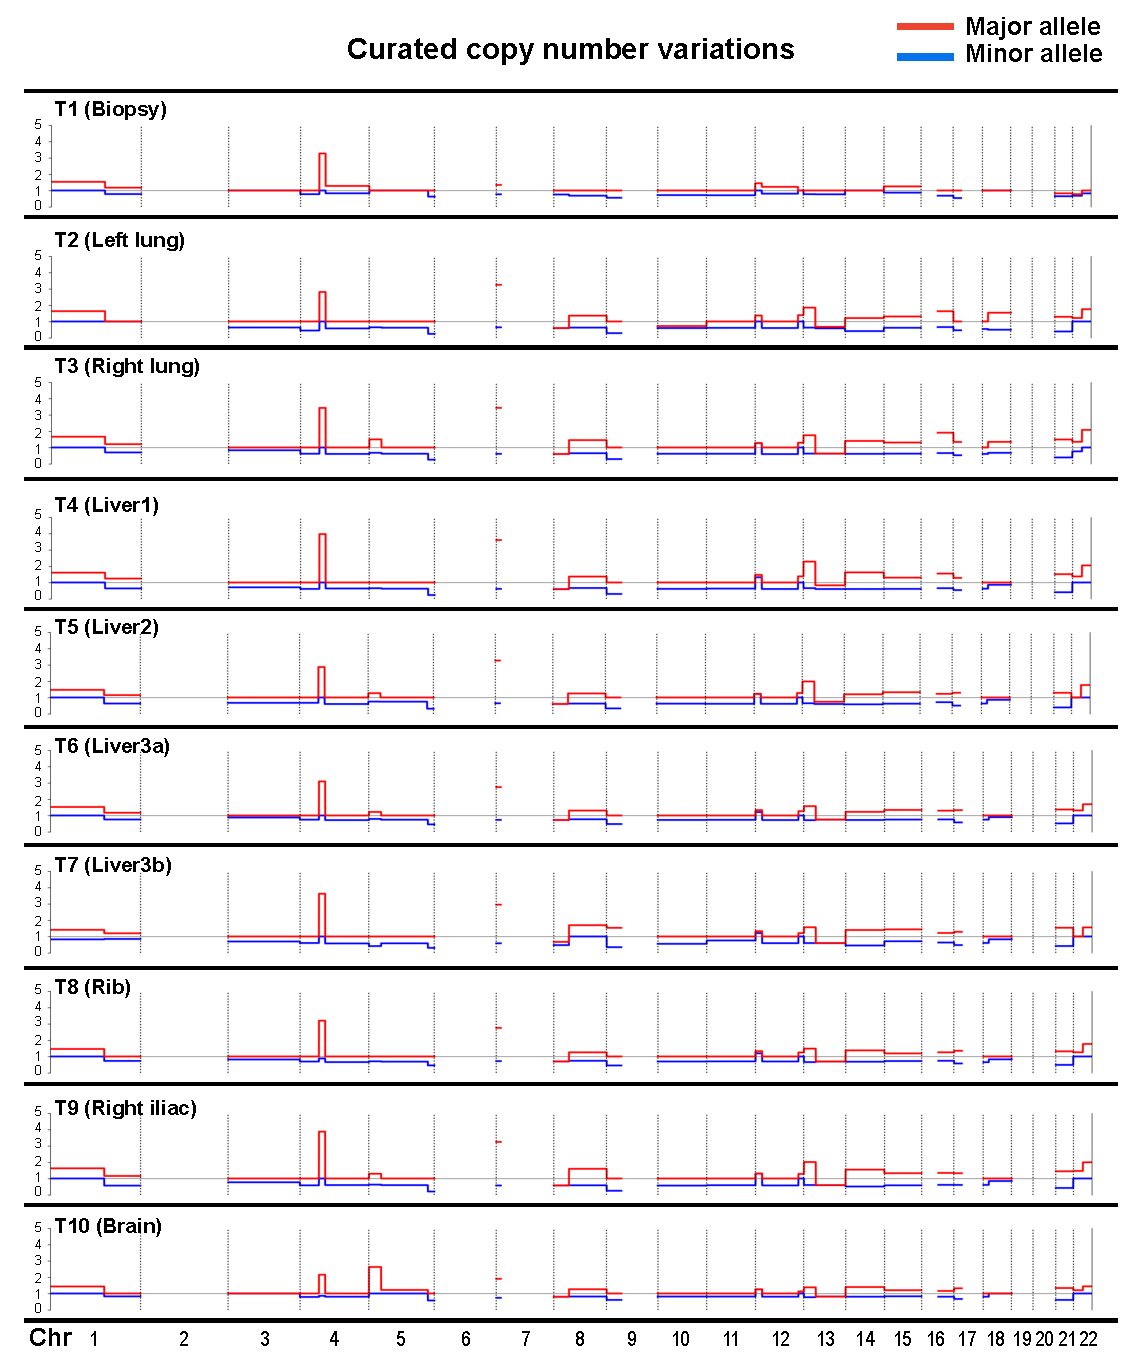
\includegraphics[width=0.9\textwidth,keepaspectratio]{images/303/cnv_plots}
    \end{center}
    \caption[Curated copy number variations per tumor sample.]{Curated copy number variations per tumor sample. Copy number variations (CNVs) were called with FALCON, and manually curated on a per-sample basis. The copy number of the major allele (red) and minor allele (blue) is depicted for each tumor sample. Areas without a listed allele are copy-neutral.}
    \label{fig:303:cnv_plots}
\end{figure}
